\documentclass[xcolor=dvipsnames,serif,10pt]{beamer}
\usepackage{etex}

\usepackage{beamerthemesplit}
\usepackage{graphics}
\usepackage{graphicx}
\usepackage{hyperref}
\usepackage[normalem]{ulem}
%\usefonttheme{professionalfonts}
%\usepackage{times}
\usepackage{tikz}
\usepackage{amsmath,cancel}
\usepackage{mathtools}
\usepackage{verbatim}
\usetikzlibrary{arrows,shapes}
\usepackage{listings}
\usepackage[]{geometry}
\usepackage{ifxetex}
\ifxetex{%
  \usepackage{fontspec}
  \setmainfont{Linux Libertine O} % or any font on your system
  \newfontfamily\quotefont[Ligatures=TeX]{Linux Libertine O} % or any font on your system
\else
  \usepackage[T1]{fontenc}
  \usepackage{libertine} % or any other font package (or none)
  \newcommand*\quotefont{\fontfamily{fxl}} % selects Libertine for quote font
\fi
\usepackage{framed}

\usepackage{soul}
\usetikzlibrary{calc}
\usetikzlibrary{decorations.pathmorphing}
\usetikzlibrary{calc,shapes.callouts,shapes.arrows}
\makeatletter

\newcommand{\defhighlighter}[3][]{%
  \tikzset{every highlighter/.style={color=#2, fill opacity=#3, #1}}%
}

\defhighlighter{yellow}{.5}

\newcommand{\highlight@DoHighlight}{
  \fill [ decoration = {random steps, amplitude=1pt, segment length=15pt}
        , outer sep = -15pt, inner sep = 0pt, decorate
        , every highlighter, this highlighter ]
        ($(begin highlight)+(0,8pt)$) rectangle ($(end highlight)+(0,-3pt)$) ;
}

\newcommand{\highlight@BeginHighlight}{
  \coordinate (begin highlight) at (0,0) ;
}

\newcommand{\highlight@EndHighlight}{
  \coordinate (end highlight) at (0,0) ;
}

\newdimen\highlight@previous
\newdimen\highlight@current

\DeclareRobustCommand*\highlight[1][]{%
  \tikzset{this highlighter/.style={#1}}%
  \SOUL@setup
  %
  \def\SOUL@preamble{%
    \begin{tikzpicture}[overlay, remember picture]
      \highlight@BeginHighlight
      \highlight@EndHighlight
    \end{tikzpicture}%
  }%
  %
  \def\SOUL@postamble{%
    \begin{tikzpicture}[overlay, remember picture]
      \highlight@EndHighlight
      \highlight@DoHighlight
    \end{tikzpicture}%
  }%
  %
  \def\SOUL@everyhyphen{%
    \discretionary{%
      \SOUL@setkern\SOUL@hyphkern
      \SOUL@sethyphenchar
      \tikz[overlay, remember picture] \highlight@EndHighlight ;%
    }{%
    }{%
      \SOUL@setkern\SOUL@charkern
    }%
  }%
  %
  \def\SOUL@everyexhyphen##1{%
    \SOUL@setkern\SOUL@hyphkern
    \hbox{##1}%
    \discretionary{%
      \tikz[overlay, remember picture] \highlight@EndHighlight ;%
    }{%
    }{%
      \SOUL@setkern\SOUL@charkern
    }%
  }%
  %
  \def\SOUL@everysyllable{%
    \begin{tikzpicture}[overlay, remember picture]
      \path let \p0 = (begin highlight), \p1 = (0,0) in \pgfextra
        \global\highlight@previous=\y0
        \global\highlight@current =\y1
      \endpgfextra (0,0) ;
      \ifdim\highlight@current < \highlight@previous
        \highlight@DoHighlight
        \highlight@BeginHighlight
      \fi
    \end{tikzpicture}%
    \the\SOUL@syllable
    \tikz[overlay, remember picture] \highlight@EndHighlight ;%
  }%
  \SOUL@
}
\makeatother


% wrap everything in its own environment
\newenvironment{shadequote}%
{\begin{quote}\openquote}
{\hfill\closequote\end{quote}}

\newcommand{\arrowthis}[2]{
        \tikz[remember picture,baseline]{\node[anchor=base,inner sep=0,outer sep=0]%
        (#1) {\underline{#1}};
        \node[overlay,single arrow,draw=none,fill=red!50,anchor=tip,rotate=60] 
        at (#1.south) {#2};}%
    }%

\newcommand{\speechthis}[2]{
        \tikz[remember picture,baseline]{\node[anchor=base,inner sep=0,outer sep=0]%
        (#1) {\underline{#1}};\node[overlay,ellipse callout,fill=blue!50] 
        at ($(#1.north)+(-.5cm,0.8cm)$) {#2};}%
    }%

\newcommand{\bubblethis}[2]{
        \tikz[remember picture,baseline]{\node[anchor=base,inner sep=0,outer sep=0]%
        (#1) {\underline{#1}};\node[overlay,cloud callout,callout relative pointer={(0.2cm,-0.7cm)},%
        aspect=2.5,fill=yellow!90] at ($(#1.north)+(-0.5cm,1.6cm)$) {#2};}%
    }%

\newcommand{\pointthis}[2]{
        \tikz[remember picture,baseline]{\node[anchor=base,inner sep=0,outer sep=0]%
        (#1) {\underline{#1}};\node[overlay,rectangle callout,%
        callout relative pointer={(0.2cm,0.7cm)},fill=green!50] at ($(#1.north)+(-.5cm,-1.4cm)$) {#2};}%
        }%


\usetikzlibrary{mindmap,backgrounds}

    \definecolor{listcomment}{rgb}{0.0,0.5,0.0}
    \definecolor{listkeyword}{rgb}{0.0,0.0,0.5}
    \definecolor{listnumbers}{gray}{0.65}
    \definecolor{listlightgray}{gray}{0.9}
    \definecolor{listwhite}{gray}{1.0}


\usetheme[secheader]{Boadilla}
\useoutertheme{miniframes}
\useinnertheme{circles}
\usecolortheme{myct}
\usepackage[latin1]{inputenc}

\graphicspath{{Figures/}{../Figures/}}

\setlength{\tabcolsep}{1pt}

\newcommand\fontvi{\fontsize{6}{8}\selectfont}
\newcommand{\ColIndent}{\hspace{\labelwidth}\hspace{\labelsep}\hspace{\labelsep}\hspace{\labelsep}\hspace{\labelsep}}

\usetikzlibrary{backgrounds}
\usetikzlibrary{positioning}
\makeatletter


%%%%%%%%%%%%%%%%%%%%%%%%%%%%%
%%  Title slide
%%%%%%%%%%%%%%%%%%%%%%%%%%%%%

% -My goal is to not get you excited about {\em my} research and the research I'm doing with
%  my collaborators.  Rather I want to get you excited about resources here at UVa for doing
%  {\em your} research, particularly if it involves computational image analysis and moderate
%  to large sized cohorts

\title[Big$\times$(Science $+$ Imaging) at UVA]{$\text{Big}\times(\text{Science}+\underbracket{\cancel{\text{Data}}}_{\small \text{Imaging}})$ @ UVA}
\author[N. Tustison]{%
  Nick Tustison, DSc
  }
\date[SOM Research Retreat]{}
\institute[ntustison@virginia.edu]{}

%\pgfdeclaremask{fsu}{fsu_logo_ybkgrd}
%\pgfdeclareimage[width=1cm]{logo}{ants_logo}
%\logo{\vbox{\vskip0.1cm\hbox{\pgfuseimage{logo}}}}

%\logo{
%  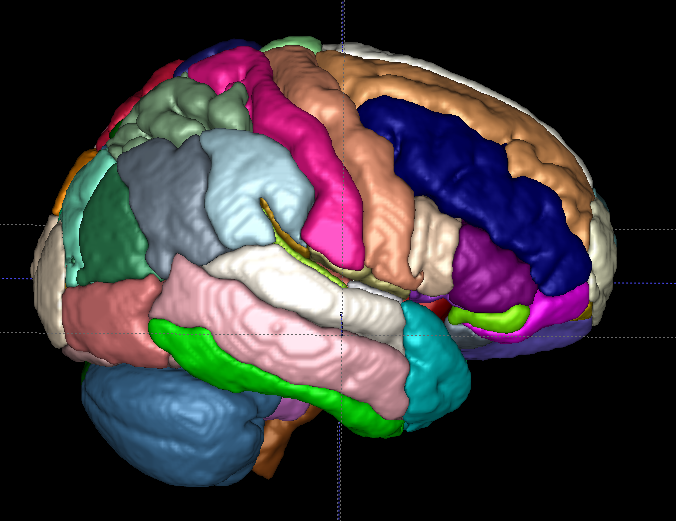
\includegraphics[height=0.8cm]{brain2.png}
%  
\includegraphics[height=0.8cm]{itkLogo.jpg}
%  }

\begin{document}

\tikzstyle{every picture}+=[remember picture]

\frame{\titlepage}



%%%%%%%%%%%%%%%%%%%%%%%%%%%%%
%%  * PNAS VBM study of London cab drivers.
%%  * 465 data points age ~ 1 + cortical_atrophy
%%%%%%%%%%%%%%%%%%%%%%%%%%%%%

% (Transition)  Let's start off with an interesting study that was done about 10 years ago.

% These computational techniques have proven invaluable in exploring fundamental, and perhaps 
% not so fundamental, neuroscience questions.

\footnotesize

\begin{frame}{Hippocampal growth in London taxi drivers}

  \begin{columns}[c]
    \begin{column}{0.5\textwidth}
    \begin{center}  
      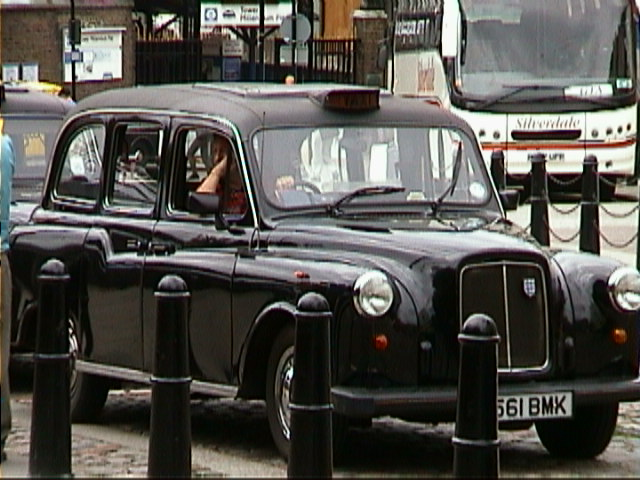
\includegraphics[width=5cm]{London_taxi.jpg}
    \end{center}
    \end{column}  
    \begin{column}{0.4\textwidth}
    \begin{center}  
      \vspace{-0.5cm}
      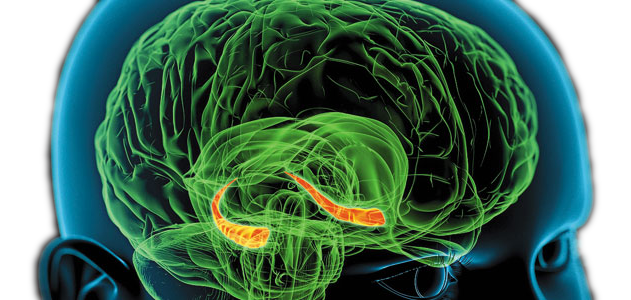
\includegraphics[width=5cm]{hippocampus.png} \\
      \pause
        \begin{align*}
			  SPM (1995):\,\,&   6418\,\,\text{citations}\\
			  VBM (2000):\,\,&   3593\,\,\text{citations}\\
			  Opt. VBM (2001):\,\,&  2353\,\,\text{citations}\\
			  TBSS (2006):\,\,&  1106\,\,\text{citations}\\
			  \end{align*}
      \vspace{0cm}
			  \highlight[yellow!100!black]{$6418 + 3593 + 2353 + 1106 = 13470\,\,\text{citations}$}
    \end{center}
    \end{column}  
  \end{columns}    
\end{frame}

\normalsize



%%%%%%%%%%%%%%%%%%%%%%%%%%%%%
%%  Studies at UVA
%%%%%%%%%%%%%%%%%%%%%%%%%%%%%

% (Transition)  Let's fast forward about 10 years to a young researcher at UVa who.
% Needless to say it was an interesting two year journey which finally ended in November
% when our paper was finally published in Human Brain Mapping which shows how these 
% techniques are susceptible to a methodological flaw known as logical circularity.



{
\usebackgroundtemplate{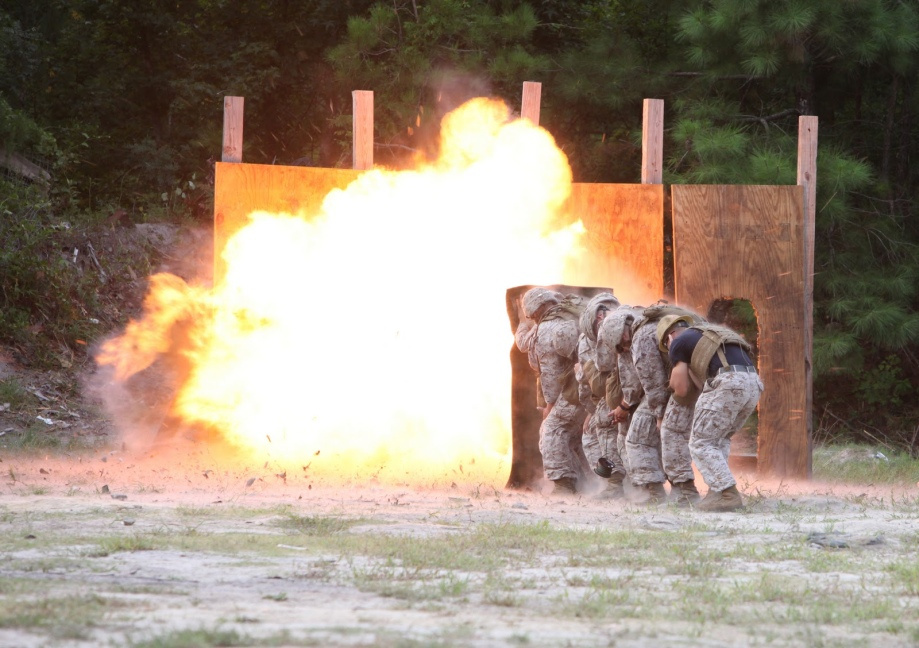
\includegraphics[width=1.175\paperwidth]{breachers.jpg}}%
\begin{frame}{TBI in breachers---{\em neuroimaging correlates?}}
   \begin{center}
   \vspace{0cm}
  \pause
   \color{black}{Investigate white matter injury \\
   {\scriptsize controls/students/instructors}} \\
   \vspace{1cm}
  \pause
   \color{black}{\em Logical circularity in\\ SPM, VBM, \& TBSS} \\
   \end{center}
\end{frame}
}


%%%%%%%%%%%%%%%%%%%%%%%%%%%%%
%%  Intro
%%%%%%%%%%%%%%%%%%%%%%%%%%%%%

% Make commands for the quotes
\newcommand*{\openquote}{\tikz[remember picture,overlay,xshift=-20pt,yshift=-5pt]
     \node (OQ) {\quotefont\fontsize{60}{60}\selectfont``};\kern0pt}
\newcommand*{\closequote}{\tikz[remember picture,overlay,xshift=-30pt,yshift=-10pt]
     \node (CQ) {\quotefont\fontsize{60}{60}\selectfont''};}
% select a colour for the shading

\begin{frame}{}
  \begin{center}

  \begin{columns}[c]
    \begin{column}{0.6\textwidth}
	    \begin{center}  
					\begin{shadequote}
					{\large {\em Maximum efficiency with minimum} wasted {\em effort}}.\par{Jigaro Kano$'$}
					\end{shadequote}
			\end{center}		
    \end{column}
    \hspace{-2.5cm}
    \begin{column}{0.2\textwidth}
		  \begin{center}
		    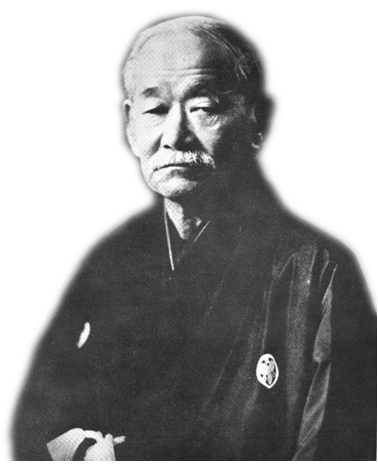
\includegraphics[height=4cm]{Kano_Jigoro.png}
		  \end{center}
		\end{column}  
  \end{columns}		
  \vspace{1cm}
  \pause
  {\LARGE \em There are \highlight[green, draw=blue]{life-altering} and \highlight[red!100!black]{free} UVA resources that you are probably not using!}
  \end{center}
\end{frame}


%%%%%%%%%%%%%%%%%%%%%%%%%%%%%
%%  What is data analysis? (neuroscience highlighted)
%%%%%%%%%%%%%%%%%%%%%%%%%%%%%

%\begin{frame}
%
%
%\tikzset{level 1 concept/.append style={font=\sf, sibling angle=135,level distance = 25mm}}
%\tikzset{level 2 concept/.append style={font=\sf, sibling angle=60,level distance = 15mm}}
%\tikzset{level 3 concept/.append style={font=\sf, sibling angle=60,level distance = 15mm}}
%\tikzset{every node/.append style={scale=0.5}}
%
%\begin{center}
%\resizebox{9cm}{7.5cm}{
%\begin{tikzpicture}
%  \path[mindmap,concept color=red!50!black,text=white]
%    node[concept,scale=0.9] {\Large Data Analysis}
%    [clockwise from=45]
%    child[concept color=green!50!black, yshift=-0.5cm] {
%      node[concept,scale=1.1] {Imaging Applications}
%      [clockwise from=120]
%      child[concept color=green!80!black] { node[concept] (ns) {Neuro\-science} }
%      child { node[concept] {Func. Lung Imaging} }
%      child { node[concept] {Breast} }
%      child { node[concept] {Cardiac} }
%    }  
%    child[concept color=blue!80!black, yshift=0.25cm] {
%      node[concept,scale=1.1] (stat) {Statistics}
%      [clockwise from=-60]
%      child { node[concept] {Linear Modeling} }
%      child { node[concept] (ml) {Machine Learning} }
%    }
%    child[concept color=orange, yshift=-0.5cm] { 
%      node[concept,scale=1.1] {Computer Science} 
%        [clockwise from=-145]
%        child { node[concept] (ad) {Algorithm Development}
%           [clockwise from=-60]
%           child { node[concept] (antsr) {\footnotesize ANTsR} }
%           child { node[concept] {ANTs} }
%           child { node[concept] {ITK} }
%           }
%        child { node[concept] (cp) {Computer Programming} }
%        child { node[concept] (cc) {Cluster Computing} }
%    };
%    
%		\newcommand{\connbluetoorange}{to[circle connection bar switch color=from (blue!80!black) to (orange)]}
%		\newcommand{\connorangetoorange}{to[circle connection bar switch color=from (orange) to (orange)]}
%		\newcommand{\conngreentoorange}{to[circle connection bar switch color=from (green!80!black) to (orange)]}
%
%  \begin{pgfonlayer}{background}
%      \path (ad) \connorangetoorange (cp);
%      \path (stat) \connbluetoorange (antsr);
%      \path (ns) \conngreentoorange (cc);
%  \end{pgfonlayer}
%    
%%  \begin{pgfonlayer}{background}
%%      \path (ml) \connbluetoorange (cs);
%%  \end{pgfonlayer}
%      
%\end{tikzpicture}
%}
%\end{center}
%\end{frame}

%%%%%%%%%%%%%%%%%%%%%%%%%%%%%
%%  Wintermark studies
%%%%%%%%%%%%%%%%%%%%%%%%%%%%%

\begin{frame}{}
\setbeamercovered{invisible}

\tikzstyle{mybox} = [draw=black, fill=bottomcolour, thick,
    rectangle, rounded corners, inner sep=10pt, inner ysep=10pt]
\tikzstyle{mybox2} = [draw=black, fill=middlecolour, thick,
    rectangle, rounded corners, inner sep=5pt, inner ysep=5pt, 
    minimum height=4cm]
\tikzstyle{fancytitle} =[fill=bottomcolour, text=textcolour, rectangle]
\tikzstyle{line} = [-latex',very thick,textcolour]


%\begin{center}
%\begin{tikzpicture}
%};
%\end{tikzpicture}%
%\end{center}
%\vspace{5mm}


\begin{center}
\begin{tikzpicture}[node distance = 4cm]

\node [shift={(4cm,4cm)},mybox] (max){%
  Misc. neuroimaging projects};

\uncover<1->{
\node [mybox2, text width = 3.5cm, opacity = 1] (SkullThickness) {%  
  \begin{center}
  \begin{tabular}{c}
  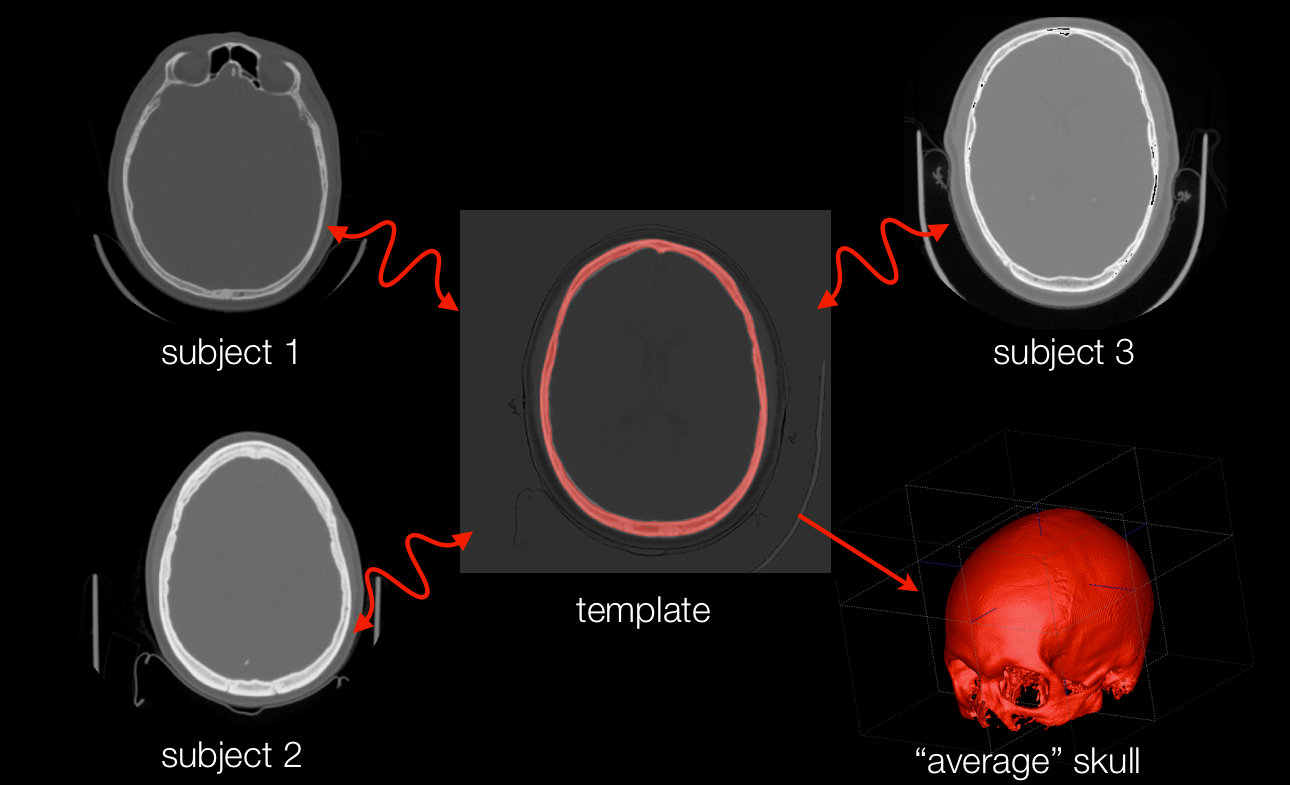
\includegraphics[height=2cm]{skullThickness.png} 
  \vspace{0.25cm}
  \end{tabular}
  \scriptsize{Surrogate CT Skull Thickness Measurements with MRI}
  \end{center}
  };
\node[fancytitle] (SkullThickness_title) at (SkullThickness.north) {\scriptsize Skull Thickness};
\path[line] (max.south) edge [out= 230, in= 90] (SkullThickness_title.north);
}


\uncover<2->{
\node [mybox2, text width = 3.5cm, right of=SkullThickness] (ET) {%
  \begin{center}
  \begin{tabular}{c}
  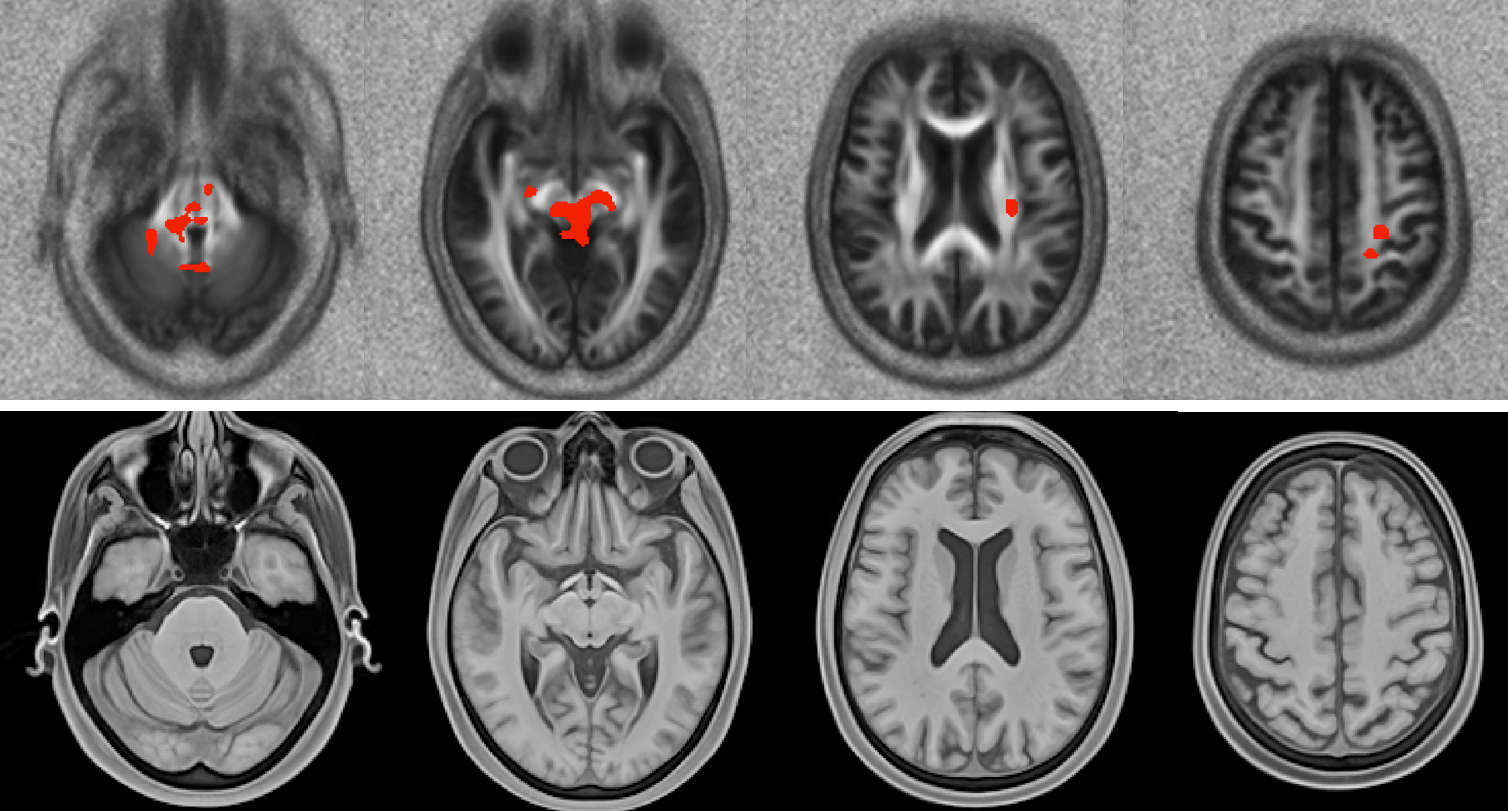
\includegraphics[height=1.8cm]{ET.png} 
  \vspace{0.25cm}
  \end{tabular}
  \scriptsize{Longitudinal FA correlations following surgical treatment for ET}
  \end{center}
  };
\node[fancytitle](ET_title) at (ET.north) {\scriptsize Essential Tremor};
 \path[line] (max.south) edge [out= 270, in= 90] (ET_title.north);
 }

\uncover<3->{
\node [mybox2, text width = 3.5cm, right of=ET] (ASL) {%
  \begin{center}
  \begin{tabular}{c}
  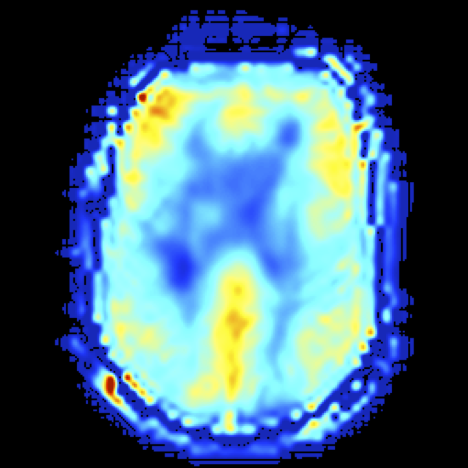
\includegraphics[height=2.5cm]{ASL.png} 
  \vspace{0.15cm}
  \end{tabular}
  \scriptsize{Automatic generation of clinical CBF maps from ASL}
  \end{center}
  };
\node[fancytitle](ASL_title) at (ASL.north) {\scriptsize ASL$\rightarrow$CBF};
\path[line] (max.south) edge [out= 310, in= 90] (ASL_title.north);
}

\end{tikzpicture}

%\begin{tikzpicture}
%  \tikz[overlay]\path[line] (max.south) edge [out= 230, in= 90] (SkullThickness_title.north);
%  \tikz[overlay]\path[line] (max.south) edge [out= 270, in= 90] (ET_title.north);
%  \tikz[overlay]\path[line] (max.south) edge [out= 310, in= 90] (ASL_title.north);
%\end{tikzpicture}
\end{center}

\end{frame}

%%%%%%%%%%%%%%%%%%%%%%%%%%%%%
%%  ANTs pipeline
%%%%%%%%%%%%%%%%%%%%%%%%%%%%%

\begin{frame}{ANTs pipeline for cortical thickness estimation}

\tikzstyle{format} = [draw, thick, fill=middlecolour]
\tikzstyle{format2} = [draw, thin, fill=middlecolour]
\tikzstyle{medium} = [ellipse, draw, thin, fill=green!20, minimum height=2.5em]
\tikzstyle{line} = [-latex',very thick,textcolour]

\usetikzlibrary{calc,decorations.pathmorphing,patterns}
\pgfdeclaredecoration{penciline}{initial}{
    \state{initial}[width=+\pgfdecoratedinputsegmentremainingdistance,
    auto corner on length=1mm,]{
        \pgfpathcurveto%
        {% From
            \pgfqpoint{\pgfdecoratedinputsegmentremainingdistance}
                      {\pgfdecorationsegmentamplitude}
        }
        {%  Control 1
        \pgfmathrand
        \pgfpointadd{\pgfqpoint{\pgfdecoratedinputsegmentremainingdistance}{0pt}}
                    {\pgfqpoint{-\pgfdecorationsegmentaspect
                     \pgfdecoratedinputsegmentremainingdistance}%
                               {\pgfmathresult\pgfdecorationsegmentamplitude}
                    }
        }
        {%TO 
        \pgfpointadd{\pgfpointdecoratedinputsegmentlast}{\pgfpoint{1pt}{1pt}}
        }
    }
    \state{final}{}
}

\begin{center}
\begin{tikzpicture}[node distance=3cm, auto,>=latex', thick,decoration=penciline, decorate]
    % We need to set at bounding box first. Otherwise the diagram
    % will change position for each frame.
    \path[use as bounding box] (-1,0) rectangle (10,0);
    
%\uncover<1->{
    \path[->,rounded corners=0.1cm] node[format, yshift=2cm, text width=1.5cm, text height=0.0cm ] (ixi) { 
        \begin{center}
			  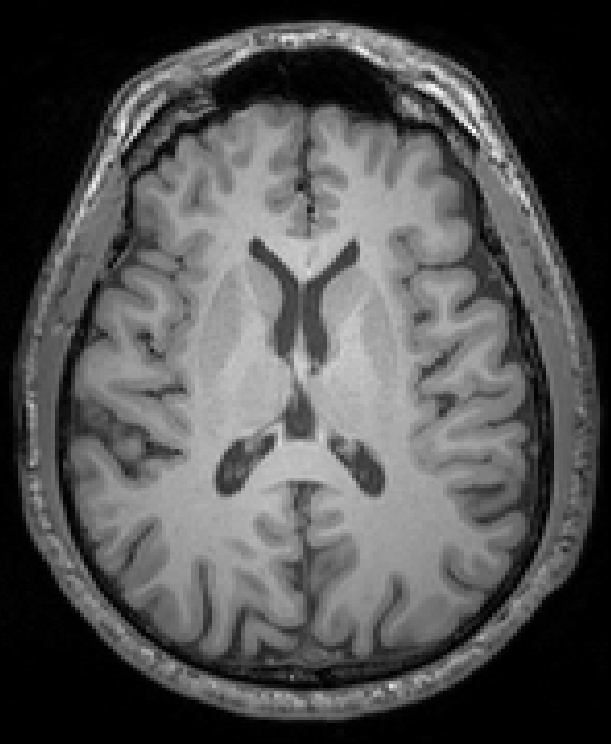
\includegraphics[height=1.75cm]{IXI221.png} \\
        \tiny{Input MRI}
        \end{center}
			  };
    \path[->] node[format, right of=ixi, xshift=0.5cm, text width=1.25cm, text height=-0.35cm ] (n4) {
          \begin{center}
            \tiny{Initial N4 bias correction}
          \end{center}
        };
    \draw[->] (ixi.0) --  (n4.180);    
    \path[->] node[format, below of=n4, yshift = 1.25cm, text width=1.25cm, text height=-0.35cm ] (be) {
          \begin{center}
            \tiny{Brain extraction}
          \end{center}
        };
    \draw[->] (n4.-90) -- (be.90);    
    \path[->] node[format, below of=be, yshift = 1.25cm, text width=1.25cm, text height=-0.35cm ] (n4_2) {
          \begin{center}
            \tiny{N4 using WM estimate}
          \end{center}
        };
    \draw[->] (be.-90) -- (n4_2.90);    
    \path[->] node[format, below of=n4_2, yshift=1.25cm, text width=1.25cm, text height=-0.35cm ] (atropos) {
          \begin{center}
            \tiny{3-tissue segmentation}
          \end{center}
        };
    \draw[->] (n4_2.-90) -- (atropos.90);    
    \path[->] node[diamond, draw, thick, fill=middlecolour, left of=atropos, xshift=1.75cm, yshift=0.875cm, text width=0.5cm, text height=-0.65cm ] (conv) {
          \begin{center}
            \tiny{Conv.?}
          \end{center}
        };
    \draw[->] (atropos.180) -| (conv.270);    
    \draw[->] (conv.90) |- node {\tiny no} (n4_2.180);    
    
    \path[->] node[format, left of=atropos, xshift=-0.5cm, text width=1.5cm, text height=-0.35cm  ] (kk) {
        \begin{center}
        \tiny{Cortical thickness estimation}
        \end{center}
			  };
    \path[->,rounded corners=0.1cm] node[format, above of=kk, yshift=-1cm, text width=1.5cm, text height=-0.3cm  ] (kkmap) {
        \begin{center}
			  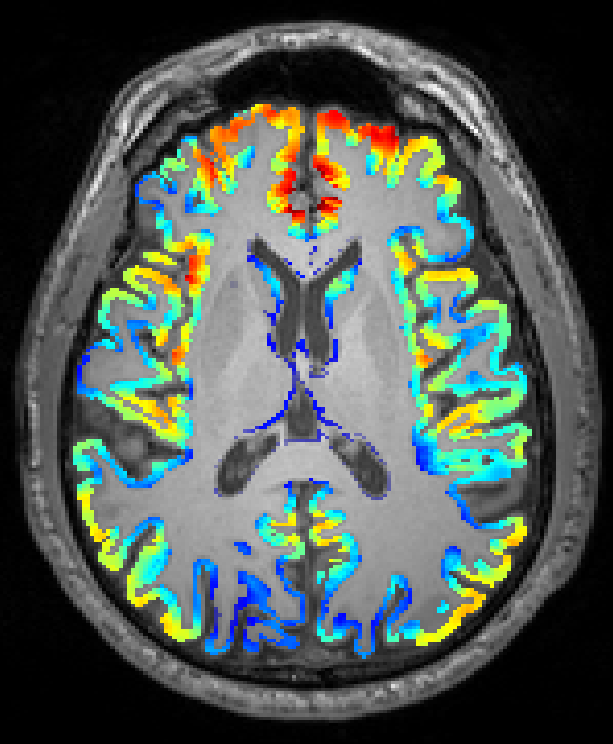
\includegraphics[height=1.75cm]{IXI221_direct.png} \\
        \tiny{Thickness map}
        \end{center}
			  };
			  
    \draw[->] (conv.180) -- node {\tiny yes} ([yshift=0cm,xshift=-0.45cm]conv.180) |- (kk.0);    
    \draw[<-] (kkmap.270) -- (kk.90);    
%}

%\uncover<2->{
    \path[->,rounded corners=0.1cm] 
      node[format, right of=n4, xshift=1.15cm, yshift=-2.5cm,text width=4.75cm,text height=-0.3cm  ] (template) { 
        \begin{center}
        \tiny{Oasis template (35 normals)}
        \begin{tabular}{cc}
          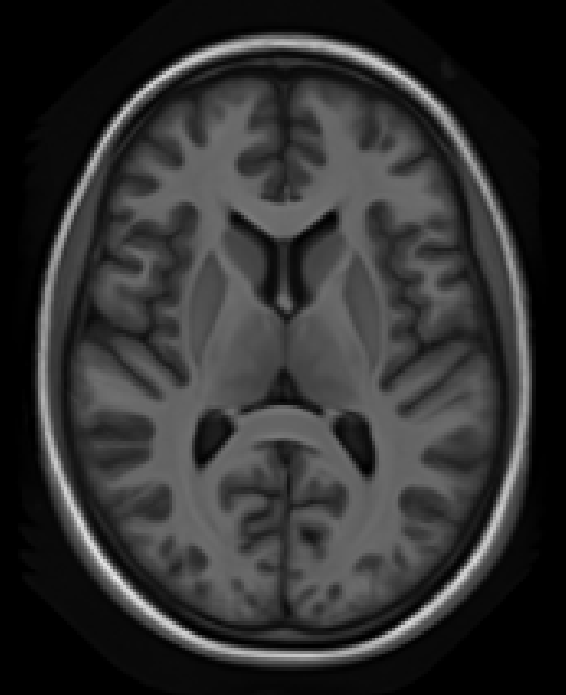
\includegraphics[width=1.5cm]{MICCAI_T1.png} &
          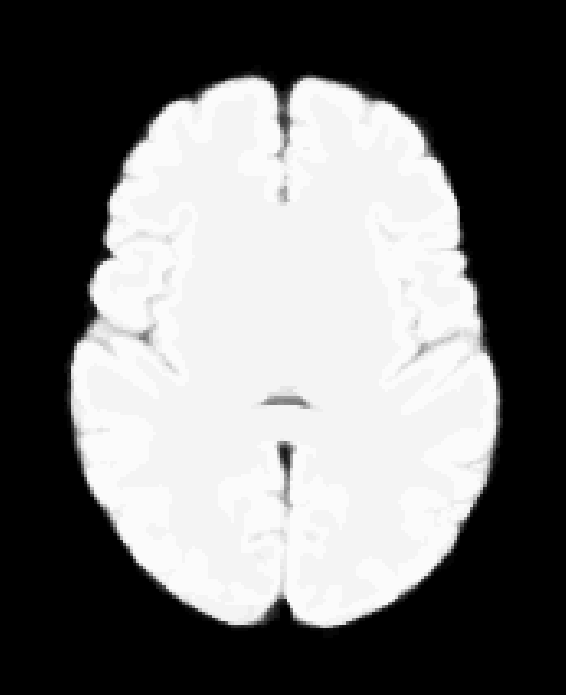
\includegraphics[width=1.5cm]{MICCAI_probMask.png} \\
          \tiny{T1} & \tiny{Whole brain} 
        \end{tabular} \\
        \begin{tabular}{ccc}
          
\includegraphics[width=1.5cm]{MICCAI_probCSF.png} &
          
\includegraphics[width=1.5cm]{MICCAI_probGM.png} &
          
\includegraphics[width=1.5cm]{MICCAI_probWM.png} \\
          \tiny{CSF} & \tiny{GM} & \tiny{WM}
        \end{tabular} \\
        \end{center}
			  };
    \draw[->,dashed] (template.160) -- ([yshift=0cm,xshift=-0.5cm]template.160) |- (be.0); 
    \draw[->,dashed] (template.200) -- ([yshift=0cm,xshift=-0.5cm]template.200) |- (atropos.0); 
%}
    
%\uncover<3->{
  \node[decorate,draw,minimum height=7.25cm,minimum width=5.65cm,dashed,rounded corners=0.2cm, thin, color = yellow] (c) at (1.7,-0.35) {};
%}  
%\uncover<4->{
  \node[decorate,draw,minimum height=5.25cm,minimum width=5.55cm,dashed,rounded corners=0.2cm, thin, color = red] (c) at (7.7,-0.45) {};
%}
\end{tikzpicture}

\end{center}

\end{frame}



%%%%%%%%%%%%%%%%%%%%%%%%%%%%%
%%  IXI Thickness
%%%%%%%%%%%%%%%%%%%%%%%%%%%%%

\begin{frame}{$\texttt{thickness} \sim 1 + \texttt{age} + \texttt{I(age\^{}2)}$}

\tikzstyle{format} = []

\begin{center}
\begin{tikzpicture}[node distance=4cm, auto,>=latex', thin]
    % We need to set at bounding box first. Otherwise the diagram
    % will change position for each frame.
    \path[use as bounding box] (-1,0) rectangle (10,0);

\uncover<1->{    
    \path[->,rounded corners=0.1cm] node[format,text width=5.5cm,xshift=1.5cm,yshift=-0.5cm ] (nirep) { 
        \begin{center}
			  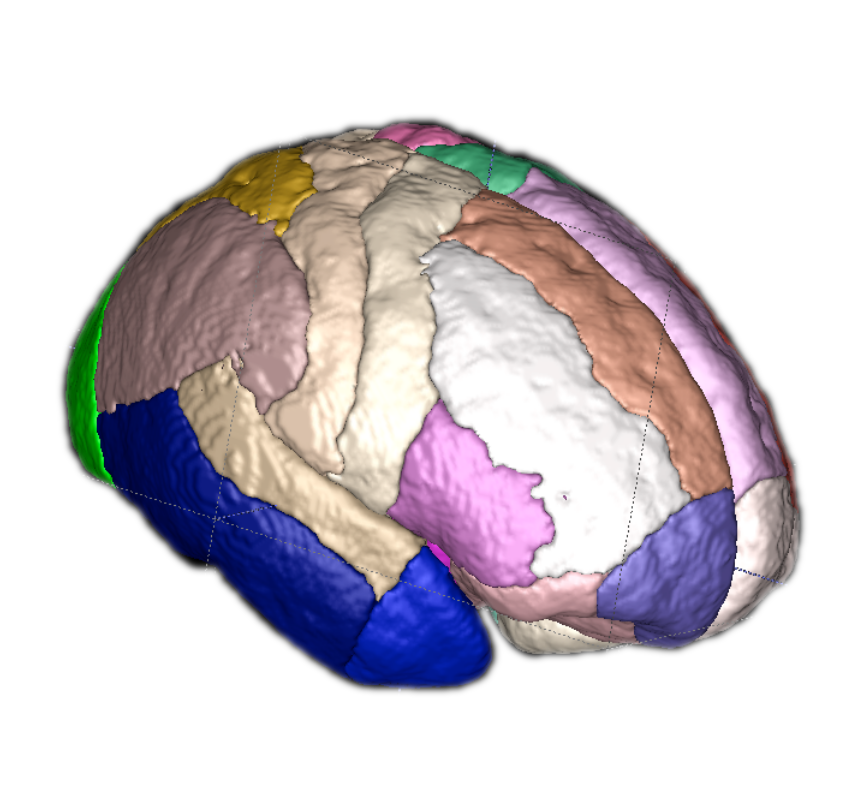
\includegraphics[width=5.5cm]{NIREPLabels.png} \\
        \end{center}
			  };
}			  
\uncover<2->{    
    \path[->,rounded corners=0.1cm] 
      node[format, right of=nirep, xshift=2.25cm, yshift=1.85cm,text width=4.5cm] (rp) {
        \begin{center}
			  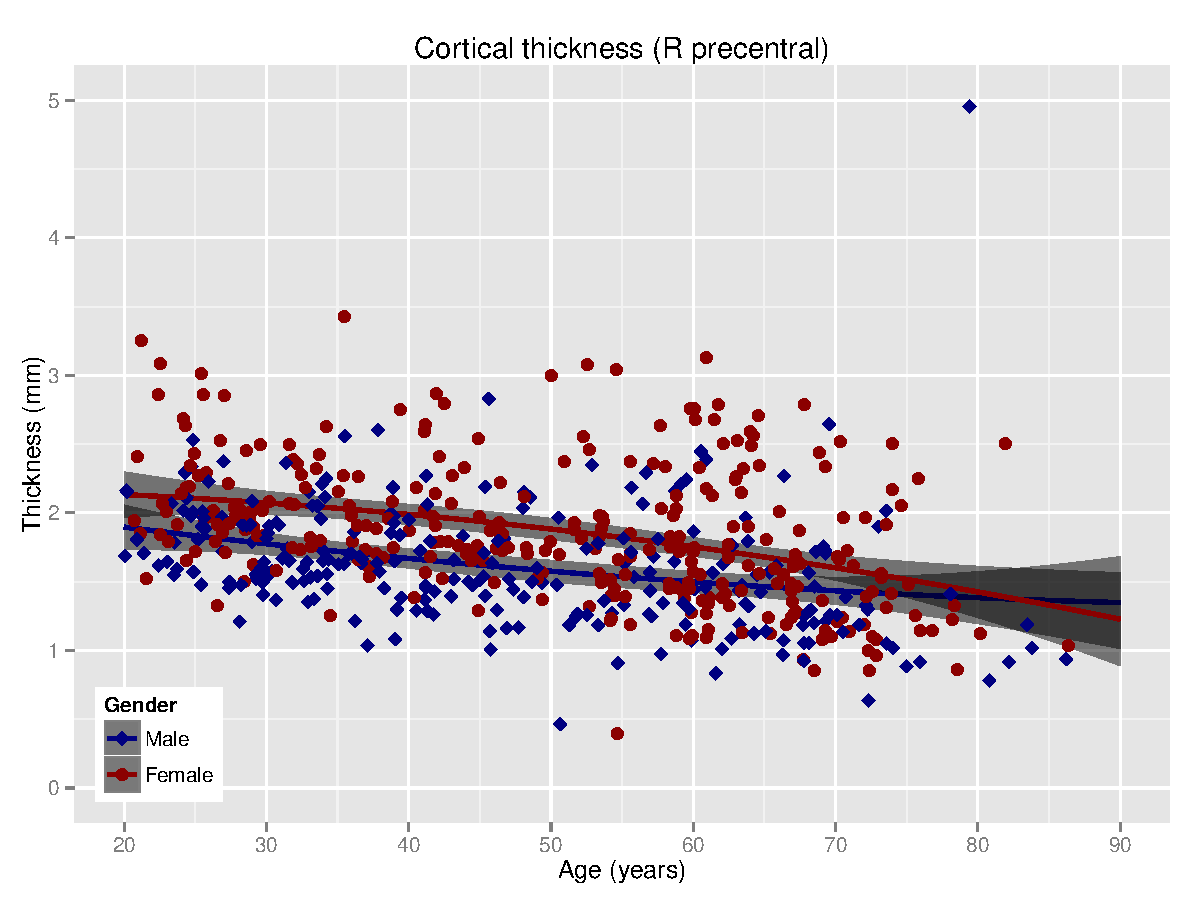
\includegraphics[width=4.5cm]{yylabel26_results.pdf}
        \end{center}
			  };
    \path[->,thick, color = yellow] (rp.west) edge [out= 180, in= 90] (1.25,0);			  
    \path[->,rounded corners=0.1cm] 
      node[format, right of=nirep, xshift=2.25cm, yshift=-1.85cm,text width=4.5cm] (rt) {
        \begin{center}
			  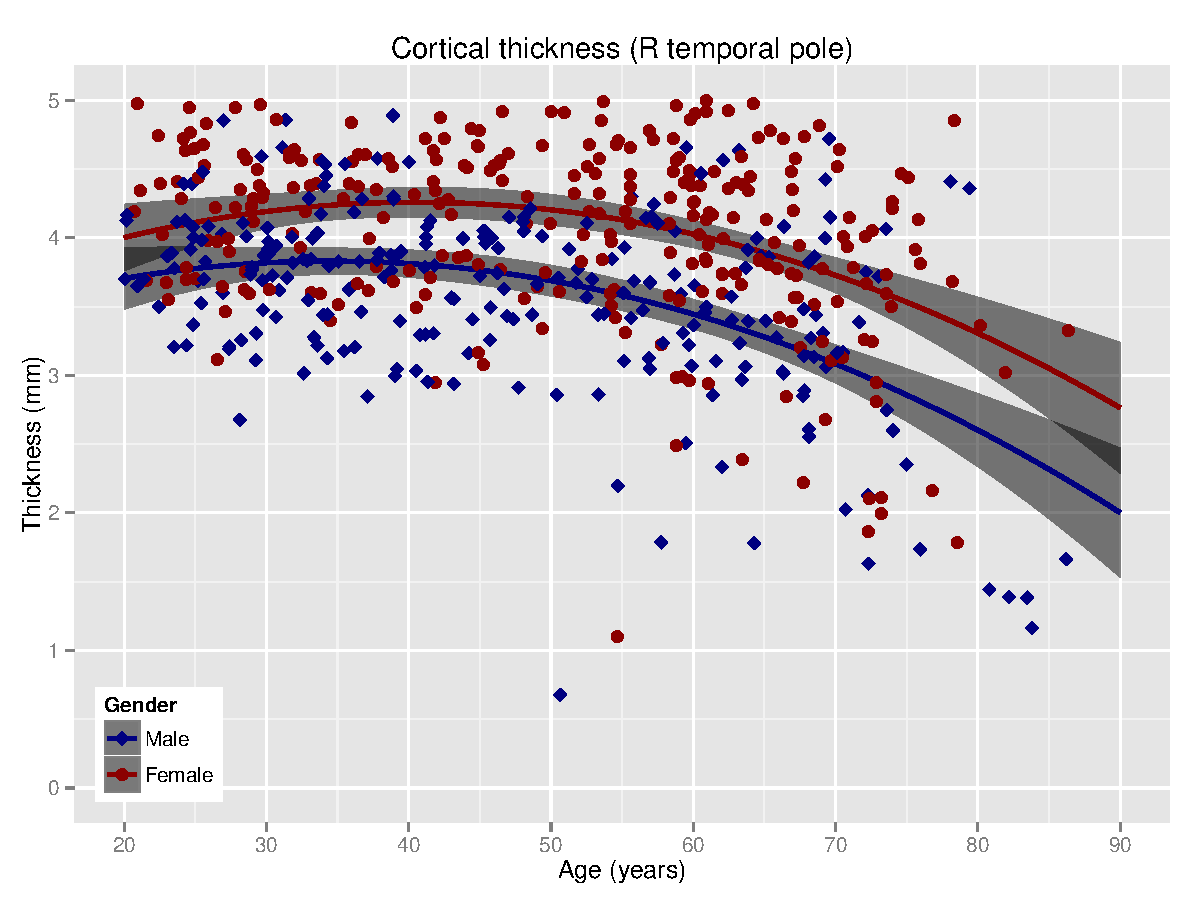
\includegraphics[width=4.5cm]{yylabel8_results.pdf} \\
        \end{center}
			  };
    \path[->,thick, color = yellow] (rt.west) edge [out= 180, in= 270] (1.4,-2.);
}			  
\uncover<3->{    
    \path[->,rounded corners=0.1cm] node[format,below of=nirep, text width = 4.0cm, yshift=1cm ] (wow) { 
        \begin{center}    
        {\color{yellow}{\em It takes $\sim$20--30 hours per subject!!}}
        \end{center}    
			  };
}			  
\end{tikzpicture}

%\begin{tikzpicture}
%  \tikz[overlay]\path[->,thick, color = yellow] (rp.west) edge [out= 180, in= 90] (-2.6,5);
%  \tikz[overlay]\path[->,thick, color = yellow] (rt.west) edge [out= 180, in= 270] (-2.5,2.75);
%\end{tikzpicture}

\end{center}

\end{frame}

%%%%%%%%%%%%%%%%%%%%%%%%%%%%%
%%  Open source software
%%%%%%%%%%%%%%%%%%%%%%%%%%%%%

% - The visible human project (1999)---one of the earliest big imaging data/big science challenges.
%

\begin{frame}{Big data $\rightarrow$ open source software}

\begin{center}
\begin{tikzpicture}[node distance=3.5cm, auto,>=latex', thin]
    % We need to set at bounding box first. Otherwise the diagram
    % will change position for each frame.
    \path[use as bounding box] (-1,0) rectangle (10,0);

\uncover<1->{
    \path[->,rounded corners=0.1cm] node[text width=5cm,xshift = 1cm] (nlm) { 
        \begin{center}
			  
\includegraphics[width=4.755cm]{visible_human_project.png} \\
        \end{center}
			  };
}			  
\uncover<2->{
    \path[->,rounded corners=0.1cm] 
        node[text width=6cm, right of=nlm, xshift=3cm, yshift=1.25cm] (logos) { 
        \begin{center}
			  
\includegraphics[width=6cm]{logos.png} \\
        \end{center}
			  };
    \path[->,rounded corners=0.1cm] node[text width=3cm, yshift=2cm, below of=logos] (itk) { 
        \begin{center}
			  
\includegraphics[width=3.cm]{ITK.png} \\
        \end{center}
			  };
}			  
\uncover<3->{
    \path[->,rounded corners=0.1cm] node[text width=2.1cm, yshift=1.2cm, below of=itk] (ants) { 
        \begin{center}
			  
\includegraphics[width=2.1cm]{ANTsLogo.png} \\
        \end{center}
			  };
}			  

\end{tikzpicture}
\end{center}
\end{frame}

%%%%%%%%%%%%%%%%%%%%%%%%%%%%%
%%  UVACSE/Linux cluster
%%%%%%%%%%%%%%%%%%%%%%%%%%%%%

\begin{frame}{UVACSE/computational cluster}

\begin{center}
\begin{tikzpicture}[node distance=2.5cm, auto,>=latex', thin]
    % We need to set at bounding box first. Otherwise the diagram
    % will change position for each frame.
    \path[use as bounding box] (-1,0) rectangle (10,0);

\uncover<1->{			  
    \path[->,rounded corners=0.1cm] node[text width=2.1cm, yshift = 2cm] (r16) { 
        \begin{center}
			  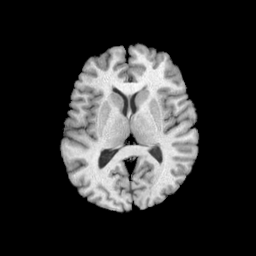
\includegraphics[width=2cm]{r16slice.png} \\
			  \vspace{-0.5cm}
			  {\footnotesize \texttt{387\_oasis}}
        \end{center}
			  };
    \path[->,rounded corners=0.1cm] node[text width=2.1cm, right of=r16] (r27) { 
        \begin{center}
			  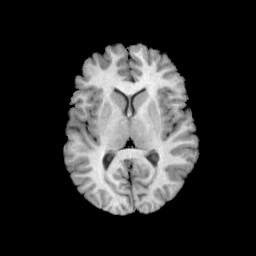
\includegraphics[width=2cm]{r27slice.png} \\
			  \vspace{-0.5cm}
			  {\footnotesize \texttt{392\_oasis}}
        \end{center}
			  };
    \path[->,rounded corners=0.1cm] node[text width=2.1cm, below of=r16] (r30) { 
        \begin{center}
			  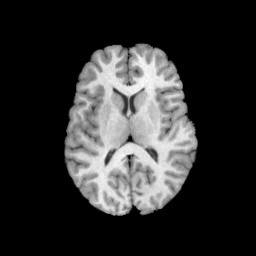
\includegraphics[width=2cm]{r30slice.png} \\
			  \vspace{-0.5cm}
			  {\footnotesize \texttt{406\_oasis}}
        \end{center}
			  };
    \path[->,rounded corners=0.1cm] node[text width=2.1cm, below of=r27] (r62) { 
        \begin{center}
			  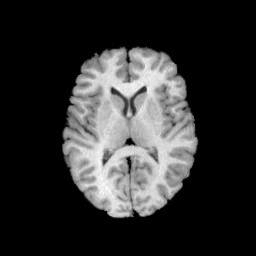
\includegraphics[width=2cm]{r62slice.png} \\
			  \vspace{-0.5cm}
			  {\footnotesize \texttt{411\_oasis}}
        \end{center}
			  };
    \path[->,rounded corners=0.1cm] node[text width=2.1cm, below of = r30] (r64) { 
        \begin{center}
			  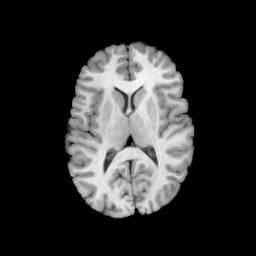
\includegraphics[width=2cm]{r64slice.png} \\
			  \vspace{-0.5cm}
			  {\footnotesize \texttt{425\_oasis}}
        \end{center}
			  };
    \path[->,rounded corners=0.1cm] node[text width=2.1cm, below of=r62] (r85) { 
        \begin{center}
			  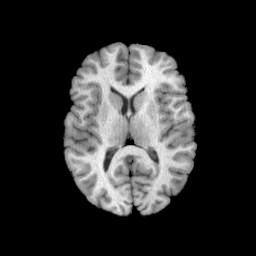
\includegraphics[width=2cm]{r85slice.png} \\
			  \vspace{-0.5cm}
			  {\footnotesize \texttt{430\_oasis}}
        \end{center}
			  };
}			  
\uncover<2->{			  
    \path[->,rounded corners=0.1cm] node[text width=6cm, xshift=2cm,right of=r62] (qstat) { 
        \begin{center}
			  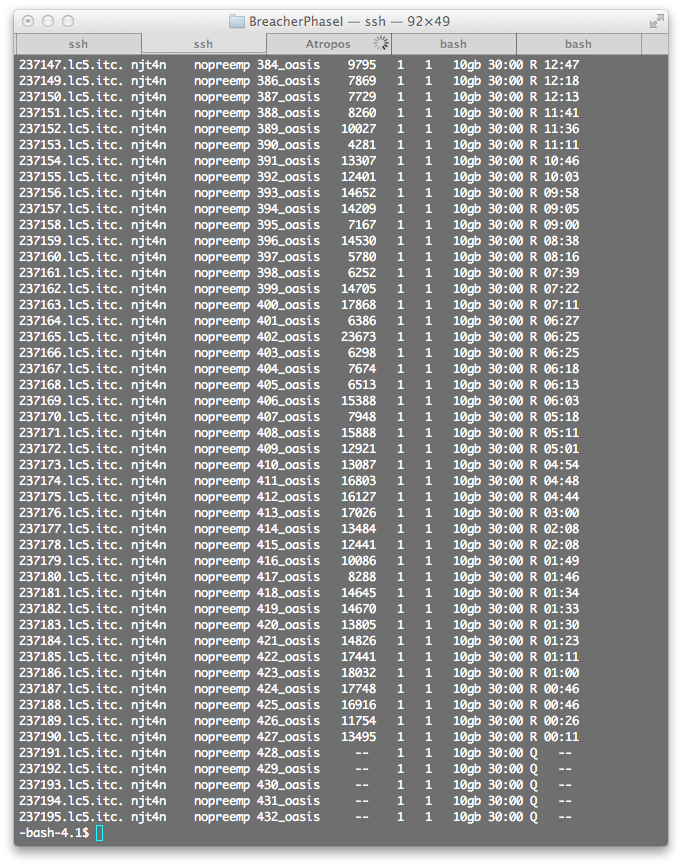
\includegraphics[width=5.75cm]{qstat.png} \\
        \end{center}
			  };		
  \path[->,thick, color = yellow, dashed] (0.5,2.3) edge [out=35,in= 145] (4.5,2.3);
  \path[->,thick, color = yellow, dashed] (3.1,1.55) edge [out=-35,in=-145] (4.5,1.55);
  \path[->,thick, color = yellow, dashed] (0.5,-0.25) edge [out=35,in= 145] (4.5,-0.25);
  \path[->,thick, color = yellow, dashed] (3.1,-0.9) edge [out=-35,in=-145] (4.5,-0.9);
  \path[->,thick, color = yellow, dashed] (0.5,-2.8) edge [out=35,in= 145] (4.5,-2.8);
  \path[->,thick, color = red, dashed] (3.1,-3.45) edge [out=-35,in=-145] (4.5,-3.45);
}  

\end{tikzpicture}

%\begin{tikzpicture}
%  \tikz[overlay]\path[->,thick, color = yellow, dashed] (-4,2.75) edge [out=35,in= 145] (0,2.75);
%  \tikz[overlay]\path[->,thick, color = yellow, dashed] (-1.4,2.1) edge [out=-35,in=-145] (0,2.1);
%  \tikz[overlay]\path[->,thick, color = yellow, dashed] (-4,0.2) edge [out=35,in= 145] (0,0.2);
%  \tikz[overlay]\path[->,thick, color = yellow, dashed] (-1.4,-0.45) edge [out=-35,in=-145] (0,-0.45);
%  \tikz[overlay]\path[->,thick, color = yellow, dashed] (-4,-2.35) edge [out=35,in= 145] (0,-2.35);
%  \tikz[overlay]\path[->,thick, color = red, dashed] (-1.4,-3.0) edge [out=-35,in=-145] (0,-3.0);
%\end{tikzpicture}

\end{center}
\end{frame}


%%%%%%%%%%%%%%%%%%%%%%%%%%%%%
%%  Closing slide
%%%%%%%%%%%%%%%%%%%%%%%%%%%%%

\begin{frame}{}


\begin{tikzpicture}[node distance=1cm, auto,>=latex', thin]
    % We need to set at bounding box first. Otherwise the diagram
    % will change position for each frame.
    \path[->,rounded corners=0.1cm] node[text width=2cm,xshift=-2cm] (ants) { 
        \begin{center}
			  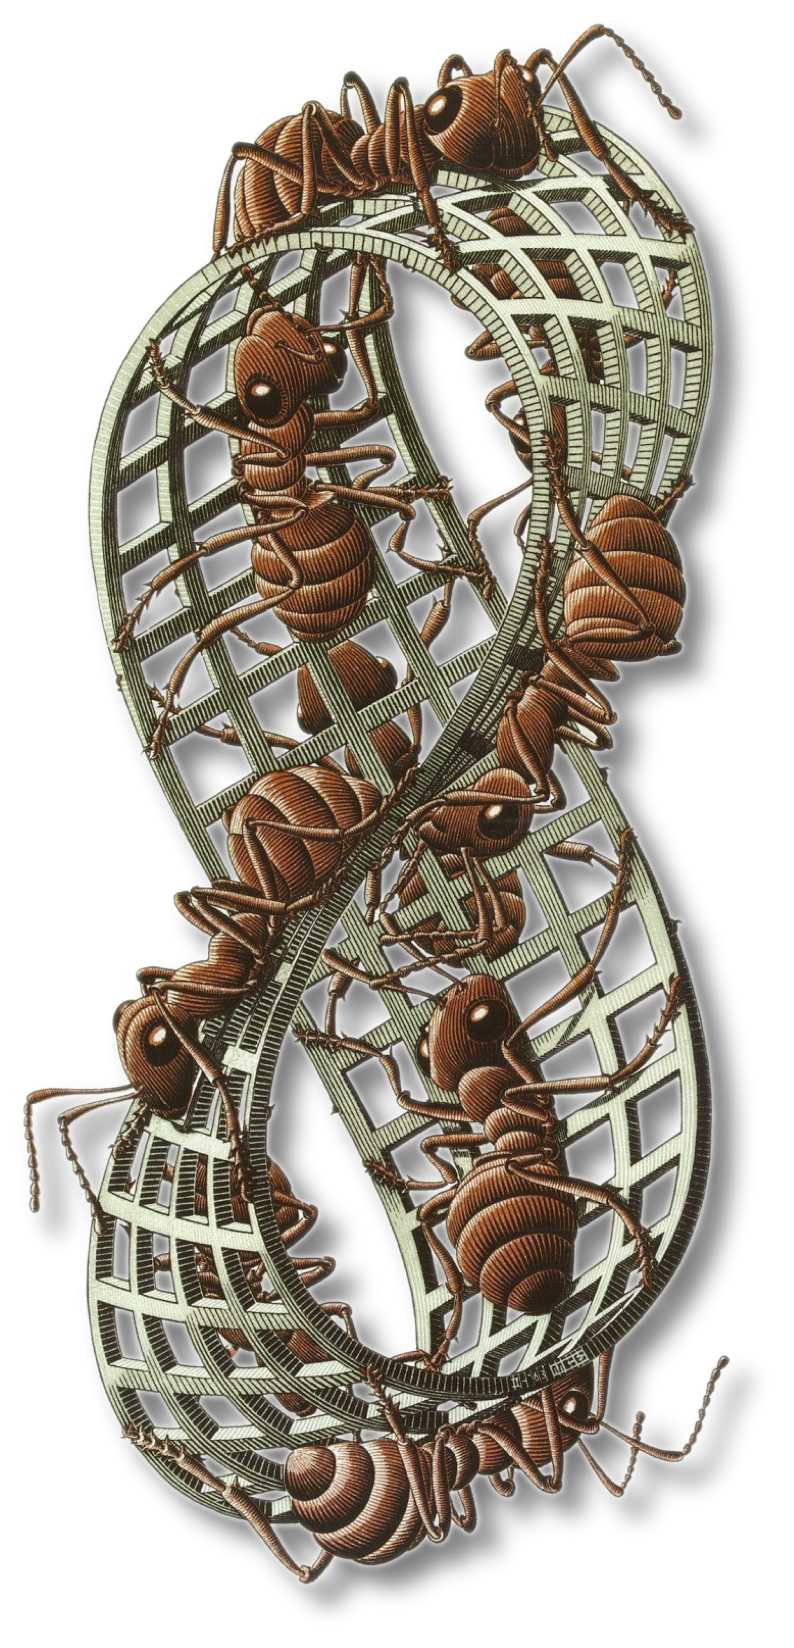
\includegraphics[width=3.5cm]{ants2.png} \\
        \end{center}
			  };
    \path[->,rounded corners=0.1cm] node[text width=7cm, xshift=5.5cm, right of=ants] { 
        \begin{center}
        \begin{block}{Further information}
        \begin{itemize}
          \item \url{http://www.itk.org}
          \item \url{http://www.picsl.upenn.edu/ANTs}
          \item \url{http://www.uvacse.virginia.edu}
        \end{itemize}
        \end{block}
        \end{center}
			  };
			  
\end{tikzpicture}
\end{frame}


\end{document}